% -*-latex-*-
% $Log: cover.tex,v $
% Revision 1.7  2001/02/08 18:53:16  boojum
% changed some \newpages to \cleardoublepages
%
% Revision 1.6  1999/10/21 14:49:31  boojum
% changed comment referring to documentstyle
%
% Revision 1.5  1999/10/21 14:39:04  boojum
% *** empty log message ***
%
% Revision 1.4  1997/04/18  17:54:10  othomas
% added page numbers on abstract and cover, and made 1 abstract
% page the default rather than 2.  (anne hunter tells me this
% is the new institute standard.)
%
% Revision 1.4  1997/04/18  17:54:10  othomas
% added page numbers on abstract and cover, and made 1 abstract
% page the default rather than 2.  (anne hunter tells me this
% is the new institute standard.)
%
% Revision 1.3  93/05/17  17:06:29  starflt
% Added acknowledgements section (suggested by tompalka)
% 
% Revision 1.2  92/04/22  13:13:13  epeisach
% Fixes for 1991 course 6 requirements
% Phrase "and to grant others the right to do so" has been added to 
% permission clause
% Second copy of abstract is not counted as separate pages so numbering works
% out
% 
% Revision 1.1  92/04/22  13:08:20  epeisach
\addcontentsline{toc}{chapter}{Cover page}
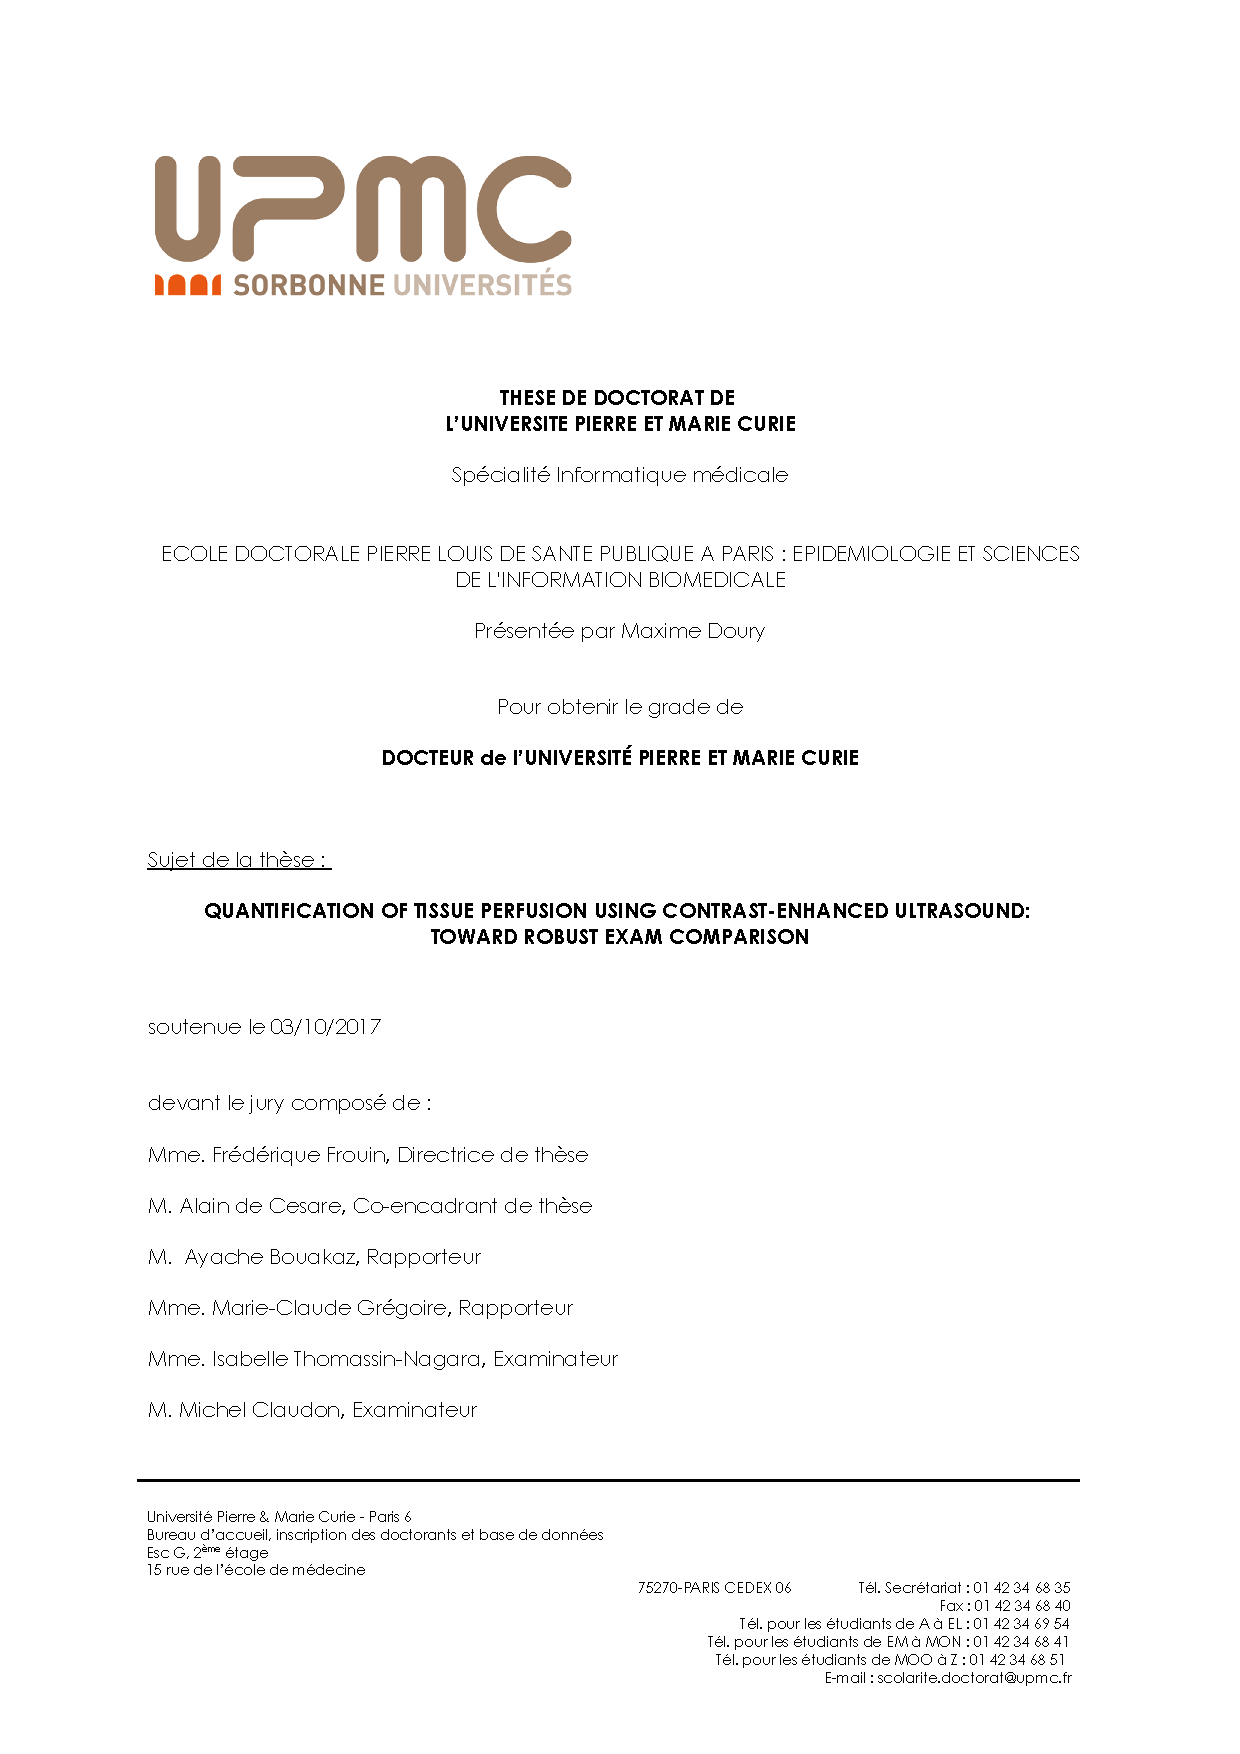
\includepdf{coverPage.pdf}
\title{Quantification of Tissue Perfusion using Contrast-Enhanced Ultrasound: 
Toward Robust Exam Comparison}
\titleFr{Quantification de la perfusion tissulaire en \'echographie de contraste: vers la comparaison robuste d'examens}
\author{Maxime Doury}
\department{Laboratoire d'Imagerie Biom\'edicale}
% If the thesis is for two degrees simultaneously, list them both
% separated by \and like this:
 \degree{Doctor of Physics}
%\degree{Bachelor of Science in Computer Science and Engineering}
\degreemonth{September}
\degreeyear{2017}
\thesisdate{September 29, 2017}

%% By default, the thesis will be copyrighted to MIT.  If you need to copyright
%% the thesis to yourself, just specify the `vi' documentclass option.  If for
%% some reason you want to exactly specify the copyright notice text, you can
%% use the \copyrightnoticetext command.  
% \copyrightnoticetext{\copyright ~Maxime Doury, 2017.}

\copyrightnoticetext{\copyright ~Maxime Doury, 2017. \\
{\footnotesize
This work is licensed under the Creative
Commons Attribution-NonCommercial 4.0
License. To view a copy of this license, visit
\url{http://creativecommons.org/licenses/by-nc/4.0} or send a
letter to
Creative Commons
543 Howard Street, 5th Floor,
San Francisco, California, 94105, USA.
}}

% If there is more than one supervisor, use the \supervisor command
% once for each.
\supervisor{Fr\'ed\'erique Frouin}{IMIV, Inserm, Paris Sud}
\cosupervisor{Alain de C\'esare}{LIB, CNRS, UPMC}

% This is the department committee chairman, not the thesis committee
% chairman.  You should replace this with your Department's Committee
% Chairman.
%\chairman{Daniel Blankschtein}{Chairman, Department Committee on Graduate Students}
\chairman{William M. Deen}{Chairman, Department Committee on Graduate Students}

% Make the titlepage based on the above information.  If you need
% something special and can't use the standard form, you can specify
% the exact text of the titlepage yourself.  Put it in a titlepage
% environment and leave blank lines where you want vertical space.
% The spaces will be adjusted to fill the entire page.  The dotted
% lines for the signatures are made with the \signature command.
% \maketitle

% The abstractpage environment sets up everything on the page except
% the text itself.  The title and other header material are put at the
% top of the page, and the supervisors are listed at the bottom.  A
% new page is begun both before and after.  Of course, an abstract may
% be more than one page itself.  If you need more control over the
% format of the page, you can use the abstract environment, which puts
% the word "Abstract" at the beginning and single spaces its text.

%% You can either \input (*not* \include) your abstract file, or you can put
%% the text of the abstract directly between the \begin{abstractpage} and
%% \end{abstractpage} commands.

% First copy: start a new page, and save the page number.
\cleardoublepage
% Uncomment the next line if you do NOT want a page number on your
% abstract and acknowledgments pages.
% \pagestyle{empty}
% \setcounter{savepage}{\thepage}
\begin{abstractpage}\addcontentsline{toc}{chapter}{Abstract}
\begin{abstractEn}
% $Log: abstract.tex,v $
% Revision 1.1  93/05/14  14:56:25  starflt
% Initial revision
%
% Revision 1.1  90/05/04  10:41:01  lwvanels
% Initial revision
%
%
%% The text of your abstract and nothing else (other than comments) goes here.
%% It will be single-spaced and the rest of the text that is supposed to go on
%% the abstract page will be generated by the abstractpage environment.  This
%% file should be \input (not \include 'd) from cover.tex.
Quantification of tissue perfusion from dynamic contrast-enhanced ultrasound data relies on appropriate modeling of the curve representing the evolution of the contrast-agent concentration inside the studied tissue.
Many factors, experimental or physiological, make inter-subject or intra-subject comparison of these perfusion parameters difficult.
In this thesis, the reproducibility and the comparison of various quantification methods was investigated through preclinical test-retest experiments and through simulations.
The investigated methods were: the log-normal model, the one-compartment model using an arterial input function, and the one-compartment model using a reference tissue.
The preclinical experiments revealed the difficulty to estimate an arterial input function directly from the image, as well as the necessity to locally correct for the time of arrival of the contrast agent in the tissue in order to ensure the model accurately fits the experimental enhancement curves.
A regularized linear estimation of the parameters of the one-compartment model using a reference tissue taking advantage of multiple tissue regions was then proposed to obtain homogeneous relative values of the tissue blood flow and tissue blood volume, expressed relatively to the parameter value inside the reference tissue.
The improved robustness and reproducibility of the method was demonstrated.
The influence of factors such as the exam duration, the sampling frequency, the number of tissue regions in the analysis, and the noise amplitude were investigated through simulations, and allowed us to formulate recommendations regarding the acquisition and the analysis of contrast-enhanced ultrasound studies.

\end{abstractEn}
\end{abstractpage}
\begin{abstractpageFr}\addcontentsline{toc}{chapter}{R\'esum\'e}
\begin{abstractFr}
% $Log: abstract.tex,v $
% Revision 1.1  93/05/14  14:56:25  starflt
% Initial revision
%
% Revision 1.1  90/05/04  10:41:01  lwvanels
% Initial revision
%
%
%% The text of your abstract and nothing else (other than comments) goes here.
%% It will be single-spaced and the rest of the text that is supposed to go on
%% the abstract page will be generated by the abstractpage environment.  This
%% file should be \input (not \include 'd) from cover.tex.
La quantification de la perfusion tissulaire \`a partir de donn\'ees dynamiques d'\'echographie de contraste repose sur une mod\'elisation appropri\'ee de la cin\'etique de la concentration en agent de contraste dans le tissu \'etudi\'e. De nombreux facteurs, exp\'erimentaux ou physiologiques, rendent la comparaison de ces param\`etres de perfusion difficile.
Dans cette th\`ese, la reproductibilit\'e et la comparaison de diff\'erentes m\'ethodes de quantification ont \'et\'e \'etudi\'ees dans le cadre d'une \'etude pr\'eclinique (test-retest) et sur des simulations num\'eriques. Les m\'ethodes \'etudies ont \'et\'e : le mod\`ele log-normal, le mod\`ele compartimental avec fonction d'entr\'ee et le mod\`ele compartimental avec tissu de r\'ef\'erence. Les \'etudes pr\'ecliniques ont montr\'e la difficult\'e d'estimation d'une fonction d'entr\'ee art\'erielle et la n\'ecessit\'e de corriger localement le temps d'arriv\'ee de l'agent de contraste dans le tissu pour que l'approximation des cin\'etiques exp\'erimentales par le mod\`ele soit de qualit\'e suffisante.
Une estimation lin\'eaire sous contrainte des param\`etres du mod\`ele compartimental avec tissu de r\'ef\'erence a \'et\'e ensuite propos\'ee pour obtenir \`a l'\'echelle r\'egionale et/ou locale des valeurs relatives coh\'erentes de d\'ebit sanguin tissulaire et de volume sanguin tissulaire, exprim\'ees par rapport aux valeurs dans le tissu de r\'ef\'erence. Il a \'et\'e montr\'e que cette approche est la plus robuste et la plus reproductible. L'influence des facteurs tels que la dur\'ee d'acquisition, la fr\'equence d'\'echantillonnage, le nombre de r\'egions utilis\'ees et l'amplitude du bruit a \'et\'e \'etudi\'ee sur des simulations et a permis de formuler des recommandations pour l'acquisition et le traitement des \'etudes en \'echographie de contraste.

\end{abstractFr}
\end{abstractpageFr}


% Additional copy: start a new page, and reset the page number.  This way,
% the second copy of the abstract is not counted as separate pages.
% Uncomment the next 6 lines if you need two copies of the abstract
% page.
% \setcounter{page}{\thesavepage}
% \begin{abstractpage}
% % $Log: abstract.tex,v $
% Revision 1.1  93/05/14  14:56:25  starflt
% Initial revision
%
% Revision 1.1  90/05/04  10:41:01  lwvanels
% Initial revision
%
%
%% The text of your abstract and nothing else (other than comments) goes here.
%% It will be single-spaced and the rest of the text that is supposed to go on
%% the abstract page will be generated by the abstractpage environment.  This
%% file should be \input (not \include 'd) from cover.tex.
In this thesis, I discuss the application and development of methods
for the automated discovery of motifs in sequential data.  These data
include DNA sequences, protein sequences, and real--valued
sequential data such as protein structures and timeseries of
arbitrary dimension. As more genomes are sequenced and annotated,
the need for automated, computational methods for analyzing
biological data is increasing rapidly.  In broad terms, the goal of
this thesis is to treat sequential data sets as unknown languages
and to develop tools for interpreting an understanding these
languages.

The first chapter of this thesis is an introduction to the
fundamentals of motif discovery, which establishes a common mode of
thought and vocabulary for the subsequent chapters.  One of the
central themes of this work is the use of grammatical models,
which are more commonly associated with the field of computational
linguistics.  In the second chapter, I use grammatical models to
design novel antimicrobial peptides (AmPs). AmPs are small proteins
used by the innate immune system to combat bacterial infection in
multicellular eukaryotes. There is mounting evidence that these
peptides are less susceptible to bacterial resistance than
traditional antibiotics and may form the basis for a novel class of
therapeutics. In this thesis, I described the rational design of
novel AmPs that show limited homology to naturally--occurring
proteins but have strong bacteriostatic activity against several
species of bacteria, including \emph{Staphylococcus aureus} and
\emph{Bacillus anthracis}. These peptides were designed using a
linguistic model of natural AmPs by treating the amino acid
sequences of natural AmPs as a formal language and building a set of
regular grammars to describe this language. This set of grammars was
used to create novel, unnatural AmP sequences that conform to the
formal syntax of natural antimicrobial peptides but populate a
previously unexplored region of protein sequence space.

The third chapter describes a novel, GEneric MOtif DIscovery
Algorithm (Gemoda) for sequential data. Gemoda can be applied to any
dataset with a sequential character, including both categorical and
real--valued data.  As I show, Gemoda deterministically discovers
motifs that are maximal in composition and length.  As well, the
algorithm allows any choice of similarity metric for finding motifs.
These motifs are representation--agnostic: they can be represented
using regular expressions, position weight matrices, or 
any other model for sequential data. I demonstrate a
number of applications of the algorithm, including the discovery of
motifs in amino acids and DNA sequences, and the discovery of
conserved protein sub--structures.

The final chapter is devoted to a series of smaller projects,
employing tools and methods indirectly related to motif discovery in
sequential data.  I describe the construction of a software tool,
Biogrep that is designed to match large pattern sets against large
biosequence databases in a \emph{parallel} fashion. This makes
biogrep well--suited to annotating sets of sequences using
biologically significant patterns.  In addition, I show that the
BLOSUM series of amino acid substitution matrices, which are
commonly used in motif discovery and sequence alignment problems,
have changed drastically over time.  The fidelity of amino acid
sequence alignment and motif discovery tools depends strongly on the
target frequencies implied by these underlying matrices.  Thus,
these results suggest that further optimization of these matrices is
possible.

The final chapter also contains two projects wherein I apply
statistical motif discovery tools instead of grammatical tools. In
the first of these two, I develop three different physiochemical
representations for a set of roughly 700 HIV--I protease substrates
and use these representations for sequence classification and
annotation.  In the second of these two projects, I develop a simple
statistical method for parsing out the phenotypic contribution of a
single mutation from libraries of functional diversity that contain
a multitude of mutations and varied phenotypes.  I show that this
new method successfully elucidates the effects of single nucleotide
polymorphisms on the strength of a promoter placed upstream of a
reporter gene.

The central theme, present throughout this work, is the development
and application of novel approaches to finding motifs in sequential
data.  The work on the design of AmPs is very applied and relies
heavily on existing literature.  In contrast, the work on Gemoda is
the greatest contribution of this thesis and contains many new
ideas.

% \end{abstractpage}



% \cleardoublepage
% \section*{Acknowledgments}\addcontentsline{toc}{chapter}{Acknowledgments}


% I am indebted to many people who both directly and indirectly
% contributed to this thesis.  First, I would like to thank those
% collaborators who directly contributed.  Most of all, I'm grateful
% for the help and friendship of Mark Styczynski. Mark was my
% collaborator on all matters computational for the past four years
% --- his influence is evident throughout this document.  I'm also
% grateful for my collaboration with Christopher Loose, who performed
% many of the experiments on antimicrobial peptides described in
% Chapter~\ref{chapter:amps}.  Finally, I would like to thank Isidore Rigoutsos, who
% straddled the line between collaborator and advisor.  Isidore taught
% me an attention to detail and a penchant for the UNIX command line
% and vi editor.

% Most importantly, I am indebted to Greg Stephanopoulos, my advisor,
% whose guidance and support was unwavering these past six years. Greg
% is the perpetual optimist --- always positive in the face of my many
% failures along the way.  He also gave me the freedom to pursue
% projects of my own choosing, which contributed greatly to my
% academic independence, if not the selection of wise projects.

% I am much obliged to my thesis committee members: my advisor Greg,
% Isidore, Bill Green, and Bob Berwick.  My committee was always
% flexible in scheduling and judicious in their application of both
% carrots and sticks.

% There are numerous people who contributed indirectly to this thesis.
% First among these is my intelligent, lovely, and vivacious wife
% Kathryn Miller--Jensen.  Next, my parents Carl and Julie, my sister
% Heather, and my in-laws, Ron, Joyce, Suzanne, Jeff, and Mindi.
% Finally, there are innumerable friends who contributed and to whom I
% am greatly appreciative including Michael Raab, Joel Moxley, Bill
% Schmitt, Vipin Guptda, and Jatin Misra.
\cleardoublepage

\section*{R\'esum\'e \'etendu}
\addcontentsline{toc}{chapter}{R\'esum\'e \'etendu}
\begin{otherlanguage}{french}
\subsection*{Titre: Quantification de la perfusion tissulaire en \'echographie de contraste: vers la comparaison robuste d'examens}

\subsection*{Introduction}
Cette th\`ese effectu\'e au sein du {\em Laboratoire d'Imagerie Biom\'edicale} (LIB) a \'et\'e financ\'e par la {\em Fondation pour la Recherche M\'edicale} (FRM).
Le projet global consiste \`a d\'evelopper un outil de classification multi-param\'etrique des tissus tumoraux exploitant diverses modalit\'es d'imagerie ultrasonore, i.e.~\'echographie quantitative, elastosonographie et \'echographie de contraste.
Les donn\'es serviront au d\'eveloppement d'un mod\`ele r\'ealiste de croissance tumorale ainsi que de la r\'eponse aux traitements anti-tumoraux.
La premi\`ere \'etape de ce projet consistait donc \`a estimer de fa\c{c}on pr\'ecis\'ement et reproductible des param\`etres de perfusion \`a partir de donn\'es de contrast ultrasonores, ce afin de les utiliser dans un contexte de suivi longitudinal.

La quantification de la perfusion est une t\^ache difficile, en effet des variations peuvent intervenir entre les examens, que ce soit au niveau exp\'erimental ou physiologique. 
Cependant ce processus s'av\`ere crucial lorsque l'on cherche \`a \'etudier la croissance de tumeurs, avec ou sans traitement.
L'imagerie de contraste permet d'\'etudier la perfusion in-vivo, cependant la comparaison quantitative d'examens reste difficile en raison du manque de reproductibilit\'e des acquisitions.
La majorit\'e des m\'ethodes de quantification de la perfusion ont \'et\'e d\'evelopp\'ees pour analyser des donn\'ees \`a une \'echelle globale, ce qui soit masque les variations spatiale de la perfusion tissulaire, soit n\'eglige les relations entre les param\`etres locaux.
Le but de cette th\`ese est de rendre l'estimation de param\`etres de perfusion robustes aux variations inter-examens, afin de rendre possible la comparaison d'examens tout en r\'ev\'elant l'h\'et\'erog\'en\'eit\'e spatiale de la fonction vasculaire.
Notre \'etude se concentre sur la quantification de l'\'echographie de contraste, cependant l'usage des m\'ethodes propos\'ees pour la quantification d'autres modalit\'es d'imagerie de contraste pourrait-\^etre \'etudi\'ee.

Le manuscrit est divis\'e en trois parties.
La premi\`ere partie cherche \`a \'etablir l'\'etat de l'art des m\'ethodes de quantification de la perfusion d\'evelopp\'ees pour les diff\'erentes modalit\'es d'imagerie de contraste.
La seconde partie \'etudie la reproductibilit\'e des param\`etres obtenus \`a l'aide de diff\'erentes approches ainsi que les relations qui les unissent, i.e.~une approche semi-quantitative, un mod\`ele \`a un compartiment utilisant une fonction d'entr\'e art\'erielle, et un mod\`le \`a un compartiment utilisant un tissus de r\'ef\'erence.
Enfin, dans la troisi\`eme partie nous pr\'esentons une nouvelle approche d'estimation du mod\`ele \`a un compartiment utilisant un tissus de r\'ef\'erence exploitant et r\'ev\'elant l'h\'et\'erog\'en\'eit\'e spatiale de la fonction vasculaire.

\subsection*{Partie I.~Quantification de la perfusion: \'etat de l'art}
Dans cette premi\`ere partie, nous \'etablissons un \'etat de l'art des m\'ethodes d\'evelopp\'ees pour quantifier la perfusion tumorale. 
Les m\'ethodes de quantification sont class\'ees en trois cat\'egories : semi-quantitatives, d\'econvolution, ou compartimentales.
Les approches semi-quantitatives extraient des param\'etres caract\'erisant la cin\'etique de la concentration en agent de contraste et sont courrament utilis\'es pour caract\'eriser la perfusion tissulaire, mais les param\`tres de ces mod\`les n'ont pas de lien direct avec la physiologie.
Les approches de d\'econvolution, ainsi que la majorit\'e des approches compartimentales, n\'ecessitent la connaissance de la fonction d'entr\'ee art\'erielle.
La fonction d'entr\'ee art\'erielle peut-\^etre obtenue par pr\'el\`evement sanguin, ou directement dans l'image. 
Cependant, les pr\'el\`evements sanguins sont invasifs, en particulier les pr\'el\`evements art\'eriels, et en raison des fortes concentrations en agent de contraste observ\'ees dans les art\`eres l'estimation directe de la fonction d'entr\'e art\'erielle dans l'image est affect\'ee par des artefacts, y compris des effets de saturation et de volumes partiels.
Les difficult\'es rencontr\'ees lors de l'estimation de la fonction d'entr\'ee art\'erielle ont motiv\'e le d\'eveloppement de m\'ethodes utilisant un tissus de r\'ef\'erence, permettant la quantification relative de la perfusion.
En effet, un tissus de r\'ef\'erence peut \^etre choisi dans une r\'egion \'etendue et bien perfus\'e de l'image, r\'eduisant ainsi les risques de saturation et de volumes partiels.
\`A notre connaissance, es mod\`eles compartimentaux, qu'ils utilisent une fonction d'entr\'e art\'erielle ou un tissus de r\'ef\'erence, ont \'et\'e appliqu\'es \`a la quantifiction de la perfusion dans la plupart des modalit\'es d'imagerie de contraste, \`a l'exception de l'\'echographie.

\subsection*{Partie II.~Reproductibilit\'e des m\'ethodes existantes et les relations entre les diff\'erentes approches}

\subsection*{Partie III.~Proposition et \'evaluation d\'une nouvelle m\'ethode de quantification}

\subsection*{Conclusion}


\end{otherlanguage}

%%%%%%%%%%%%%%%%%%%%%%%%%%%%%%%%%%%%%%%%%%%%%%%%%%%%%%%%%%%%%%%%%%%%%%
% -*-latex-*-
